\documentclass[12pt]{article}
\usepackage{framed}
\usepackage{graphicx}
\begin{document}
	
	\section*{The Data Scientist’s Toolbox - Week 3 Quiz}
	
	\subsection*{Statistical Inference}
	\begin{itemize}
		\item In statistics, statistical inference is the process of drawing conclusions from data that are subject to random variation, for example, observational errors or sampling variation.
		
		\item Initial requirements of such a system of procedures for inference and induction are that the system should produce reasonable answers when applied to well-defined situations and that it should be general enough to be applied across a range of situations. 
		\item Inferential statistics are used to test hypotheses and make estimations using sample data. Whereas descriptive statistics describe a sample, inferential statistics infer predictions about a larger population that the sample represents.
		\item 	The outcome of statistical inference may be an answer to the question "what should be done next?", where this might be a decision about making further experiments or surveys, or about drawing a conclusion before implementing some organizational or governmental policy.
	\end{itemize}
	\newpage
	
	\subsection*{Exploratory Data Analysis}
	\begin{itemize}
	\item	In statistics, exploratory data analysis (EDA) is an approach to analyzing data sets to summarize their main characteristics, often with visual methods. 
	\item A statistical model can be used or not, but primarily EDA is for seeing what the data can tell us beyond the formal modeling or hypothesis testing task. 
	\item Exploratory data analysis was promoted by John Tukey to encourage statisticians to explore the data, and possibly formulate hypotheses that could lead to new data collection and experiments. 
%	\item EDA is different from initial data analysis (IDA), which focuses more narrowly on checking assumptions required for model fitting and hypothesis testing, and handling missing values and making transformations of variables as needed. EDA encompasses IDA.
	\end{itemize}

\newpage
	% Data Scientist Toolkit Week 2 Quiz
	\subsection*{Question 1 - Types of Data Analysis}
We take a random sample of individuals in a population and identify whether they smoke and if they have cancer. We observe that there is a strong relationship between whether a person in the sample smoked or not and whether they have lung cancer. \\

\bigskip
\noindent We claim that the smoking is related to lung cancer in the larger population. We explain we think that the reason for this relationship is because cigarette smoke contains known carcinogens such as arsenic and benzene, which make cells in the lungs become cancerous.
\begin{itemize}
\item[(i)] This is an example of an inferential data analysis.
\item[(ii)] This is an example of a mechanistic data analysis.
\item[(iii)] This is an example of an descriptive data analysis.
\item[(iv)] This is an example of a causal data analysis.
\end{itemize}
%------------------------------------------------------------------------------------------%
\newpage
\subsection*{Question 2}
What is the most important thing in Data Science?
\begin{itemize}
\item[(i)] Working with large data sets.
\item[(ii)] Hacking skills.
\item[(iii)] Knowing Hadoop and Pig.
\item[(iv)] The question you are trying to answer.
\end{itemize}
%------------------------------------------------------------------------------------------%
\newpage
\subsection*{Question 3}
If the goal of a study was to relate \textit{Martha Stewart Living Subscribers} to \textit{Our Site's Users} based on the number of people that lived in each region of the US, what would be the potential problem? 

\begin{figure}[h!]
\centering
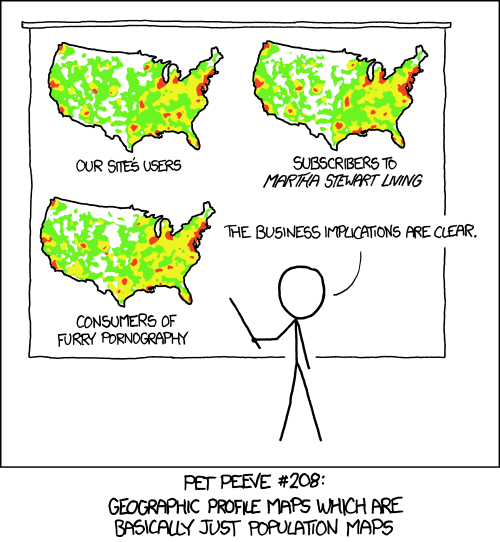
\includegraphics[width=0.7\linewidth]{datascitoolbox-heatmap}
\end{figure}

\begin{itemize}
\item[(i)] There would be confounding because the number of people that live in an area is related to both \textit{Martha Stewart Living Subscribers} and \textit{Our Site's Users}.
\item[(ii)] We would be performing inference on the relationship between \textit{Martha Stewart Living Subscribers} and \textit{Our Site's Users}.
\item[(iii)] We wouldn't know the sensitivity of our predictions.
\item[(iv)] We wouldn't be able to estimate the variability in \textit{Martha Stewart Living Subscribers}.
\end{itemize}
%------------------------------------------------------------------------------------------%
\newpage

\subsection*{Experimental Design}

\begin{itemize}
\item Experimental design is the design of any information-gathering exercises where variation is present, whether under the full control of the experimenter or not. 
%However, in statistics, these terms are usually used for controlled experiments. Formal planned experimentation is often used in evaluating physical objects, chemical formulations, structures, components, and materials. 

%Other types of study, and their design, are discussed in the articles on computer experiments, opinion polls and statistical surveys (which are types of observational study), natural experiments and quasi-experiments (for example, quasi-experimental design). 

\item 
In the design of experiments, the experimenter is often interested in the effect of some process or intervention (the "treatment") on some objects (the "experimental units"), which may be people, parts of people, groups of people, plants, animals, etc. 

\item Design of experiments is thus a discipline that has very broad application across all the natural and social sciences and engineering.
\end{itemize}
\newpage
\begin{itemize}
\item  We are concerned with the analysis of data generated from an experiment. It is wise to take time and effort to organise the experiment properly to ensure that the right type of data, and enough of it, is available to answer the questions of interest as clearly and efficiently as possible. This process is called experimental design.
\item The specific questions that the experiment is intended to answer must be clearly identified before carrying out the experiment.
\item We should also attempt to identify known or expected sources of variability in the experimental units since one of the main aims of a designed experiment is to reduce the effect of these sources of variability on the answers to questions of interest. That is, we design the experiment in order to improve the precision of our answers.
\end{itemize}
\subsubsection*{Treatment}
\begin{itemize}
\item In experiments, a treatment is something that researchers administer to experimantal units . 
\item For example, a corn field is divided into four, each part is 'treated' with a different fertiliser to see which produces the most corn; a teacher practices different teaching methods on different groups in her class to see which yields the best results; a doctor treats a patient with a skin condition with different creams to see which is most effective.
\item Treatments are administered to experimental units by 'level', where level implies amount or magnitude. For example, if the experimental units were given 5mg, 10mg, 15mg of a medication, those amounts would be three levels of the treatment. 
\item 'Level' is also used for categorical variables, such as Drugs A, B, and C, where the three are different kinds of drug, not different amounts of the same thing.
\end{itemize}
\subsubsection*{Factor}
\begin{itemize}
\item A factor of an experiment is a controlled independent variable; a variable whose levels are set by the experimenter.
\item A factor is a general type or category of treatments. Different treatments constitute different levels of a factor. For example, three different groups of runners are subjected to different training methods. The runners are the experimental units, the training methods, the treatments, where the three types of training methods constitute three levels of the factor 'type of training'.

\end{itemize}


\newpage
\subsection*{Question 4}
What is an experimental design tool that can be used to address variables that may be confounders at the design phase of an experiment?
\begin{itemize}
\item[(i)] Randomization
\item[(ii)] Only using non-confounding variables.
\item[(iii)] Using data from a database.
\item[(iv)] Using all the data you have access too.
\end{itemize}
%------------------------------------------------------------------------------------------%
\newpage
\subsection*{Question 5}
What is the reason behind the explosion of interest in big data?

\begin{itemize}
\item[(i)] We recently discovered ways to use data to make predictions.
\item[(ii)] The price and difficulty of collecting and storing data has dramatically dropped.
\item[(iii)] We recently discovered ways to use data to answer scientific and business questions.
\item[(iv)] There have been massive improvements in machine learning algorithms.
\end{itemize}
%------------------------------------------------------------------------------------------%
\end{document}